\documentclass{article}

\usepackage{amsmath}
\usepackage{amsthm}
\usepackage{mathtools}

\usepackage{graphicx}

\usepackage{cite}
\usepackage{hyperref}

\usepackage{braket}
\usepackage{diffcoeff}
\diffdef{}{op-symbol=\mathrm{d},op-order-sep=0mu}

\title{MQM Term Paper}
\author{Duarte Maia}
\date{}


\newcommand{\e}{\mathrm{e}}
\newcommand{\I}{\mathrm{i}}

\DeclareMathOperator{\re}{Re}
\DeclareMathOperator{\tg}{tg}

\begin{document}

\tableofcontents

\section{Introduction}

In both papers we were given to base our term paper on, the center of attention in regards to out-of-order time correlators is the square of the commutator $[x(t), p(0)]$, or in other words, a four-point correlation function. The direction I decided to take for this term paper was to investigate a trivial generalization of this: the $2N$-point correlators of the form $-\braket{[x(t),p(0)]^N}$, in particular I wanted to find a way to approximate these correlation functions for big $N$.

There were two major ideas I wanted to test, based on the two parts of the class I enjoyed the most. First, I tried to set up an `ordinary differential equation for large $N$', similar to when we found determinants of infinite-size matrices by interpreting a recurrence relation for large $N$ as an approximation of the solution of an ODE. Second, I tried to interpret the large $N$ limit as a path integral, upon finding an expression that looked suspiciously like the definition of path integral we learned in class. Unfortunately, neither of these ideas panned out.

This term paper has two major sections. In the first, I calculate the $2N$-point functions for three simple systems. If I knew anything about quantum or classical chaos, I might try to interpret the results I got in those terms, but unfortunately I'm flying blind. In the second section, I show my attempts at constructing the machinery I mentioned in the previous paragraphs, and, more importantly, my calculations showing that they fail.

\section{Notation and Basic Definitions}

I will mostly follow the notation of \cite{Hashimoto_2017}, which I will now describe.

We usually consider OTOCs of the form $C_T(t) = -\braket{[x(t), p]^2}$, where the braket represents a thermal average and $p = p(0)$. I will also write $x$ for the operator $x(0)$.

I studied the following generalization of the macrocanonical OTOC:
\begin{equation}
C_T^N(t) = -\braket{[x(t),p]^N}.
\end{equation}

To do so, I followed the footsteps of \cite{Hashimoto_2017} in introducing the following auxilliary quantities:
\begin{gather}
C_T^N(t) = -\frac1Z \sum \e^{-\beta E_n} c_n^N(t),\label{bigcdef}\\
c_n^N(t) = \braket{n|[x(t), p]^N|n} = \sum_{k_1, \dots, k_{N-1}} b_{nk_1} b_{k_1 k_2} \dots b_{k_{N-1} n}, \label{smallcdef}\\
b_{ij} = \braket{i|[x(t), p]|j}. \label{bdef}
\end{gather}

We refer to the quantities $c_n^N(t)$ as microcanonical OTOCs. Note that my definition of $b_{ij}$ differs by a factor of $-\I$ from the definition of \cite{Hashimoto_2017}.

In the case where $H$ has only a discrete spectrum $E_n$ with eigenvectors $\ket n$, we can write $b_{ij}$ as
\[b_{ij} = \sum_k \e^{\I (E_i - E_k) t} x_{ik} p_{kj} - \e^{\I (E_k - E_j) t} p_{ik} x_{jm},\]
and in the case where $H$ is of the form $H = \frac1{2m} p^2 + U(x)$, this can be written only in terms of the $E_n$ and matrix elements of $x$ as follows:
\begin{gather}
p_{ij} = - \frac{\I m}{\hbar} (E_i - E_j) x_{ij},\\
b_{ij} = - \frac{\I m}{\hbar} \sum_k \left( \e^{\I (E_i - E_k) t} (E_k - E_j) - \e^{\I (E_k - E_j) t} (E_k - E_j) \right) x_{ik} x_{kj}. \label{bijwithx}
\end{gather}

\section{Three trivial examples}

In this section, I will use the formulas obtained in the previous section to calculate $C_T^N(t)$ for three particular cases: the Harmonic Oscillator, the Infinite Well, and the free particle.

\subsection{The Harmonic Oscillator}

Consider the Harmonic Oscillator with Hamiltonian given by
\begin{equation}
H = \frac1{2m} p^2 + \frac12 m \omega^2 x^2.
\end{equation}

In this case, the spectrum and matrix elements of the $x$ operator are well-known
\begin{gather}
E_n = \hbar \omega (n + \tfrac12),\\
x_{ij} = \sqrt{\frac\hbar{2 \omega m}} (\sqrt{j} \delta_{i,j-1} + \sqrt{j+1} \delta_{i,j+1}), %todo check this
\end{gather}
and so we can calculate $b_{ij}$ explicitly
\begin{align*}
b_{ij} &= -\frac{\I m}{\hbar} \sum_k \begin{multlined}
\left(\e^{\I \hbar \omega (i-k) t} \hbar \omega (k - j) - \e^{\I \hbar \omega (k-j) t} \hbar \omega (i - k) \right) \times\\
\times \frac{\hbar}{2 \omega m} (\sqrt k \delta_{i, k-1} + \sqrt{k+1} \delta_{i, k+1}) (\sqrt j \delta_{k, j-1} + \sqrt{j+1} \delta_{k, j+1})\end{multlined}\\
&= - \I \hbar \cos(\hbar \omega t) \delta_{ij}.
\end{align*}

Consequently, we can easily calculate $c_n^N(t)$ and $C_T^N(t)$:
\begin{gather*}
c_n^N(t) = \sum_{k_1,\dots, k_{N-1}} b_{nk_1} b_{k_1 k_2} \dots b_{k_{N-1}n} = \left( -\I \hbar \cos(\hbar \omega t) \right)^N\\
C_T^N(t) = - \left( -\I \hbar \cos(\hbar \omega t) \right)^N.
\end{gather*}

This agrees with the results of \cite{Hashimoto_2017} for $N = 2$, as it should.

\subsection{The Infinite Well}

Let us now consider the infinite well in the interval $[-L, L]$. Instead of calculating the $b_{ij}$ coefficients analytically, I will use formula \eqref{bijwithx} to calculate them numerically using the matrix elements of $x$.

The spectrum and wavefunctions of the infinite well are known:
\begin{gather*}
E_n = \frac{\hbar^2 \pi^2 n^2}{8 m L^2}, n > 0,\\
\psi_n(x) = \begin{cases}
\frac1{\sqrt L} \cos(k_n x), & \text{$n$ odd},\\
\frac1{\sqrt L} \sin(k_n x), & \text{$n$ even},
\end{cases}\\
k_n = \frac1\hbar \sqrt{2 m E_n} = \frac{\pi n}{2 L}.
\end{gather*}

This allows us to calculate the matrix elements of $x$. Begin by writing out the definition:
\begin{equation*}
x_{ij} = \braket{i|x|j} = \frac1{L} \int_{-L}^L x \psi_i(x) \psi_j(x) \dl x.
\end{equation*}

Now, note that if $i$ and $j$ have the same parity the integrand is odd, so the only relevant case has $i$ odd and $j$ even or vice-versa. The integral can be calculated analytically, yielding
\begin{equation}
x_{ij} = \begin{cases}
\frac1{L} \int_{-L}^L x \sin(k_i x) \cos(k_j x) \dl x = \frac{16 \I^{i+j+1} L}{\pi^2} \frac{ij}{(i^2 - j^2)^2}, & \text{$i$ even, $j$ odd,}\\
-x_{ji} & \text{$i$ odd, $j$ even}\\
0 & \text{otherwise.}
\end{cases}
\end{equation}

Consequently, we can now calculate $b_{ij}$ using \eqref{bijwithx}, which we recall now:
\[b_{ij} = - \frac{\I m}{\hbar} \sum_{k>0} \left( \e^{\I (E_i - E_k) t} (E_k - E_j) - \e^{\I (E_k - E_j) t} (E_k - E_j) \right) x_{ik} x_{kj}.\]

Notice that if $i$ and $j$ have different parities, it is impossible for $x_{ik}$ and $x_{kj}$ to be non-null at the same time. Therefore, we need only look at the cases where $i$ and $j$ are both even or both odd.

If $i$ and $j$ are both even, we get
\begin{align*}
b_{ij} &= - \frac{\I m}{\hbar} \sum_{\text{$k$ odd}} \left( \e^{\I (E_i - E_k) t} (E_k - E_j) - \e^{\I (E_k - E_j) t} (E_i - E_j) \right) x_{ik} x_{kj}\\
&
\begin{multlined}
= - \frac{\I m}{\hbar} \sum_{\text{$k$ odd}} \left( \e^{\I \frac{\hbar^2 \pi^2}{8m L^2} (i^2 - k^2) t} \tfrac{\hbar^2 \pi^2}{8m L^2} (k^2 - j^2) - \e^{\I \frac{\hbar^2 \pi^2}{8m L^2} (k^2 - j^2) t} \tfrac{\hbar^2 \pi^2}{8m L^2} (i^2 - k^2) \right)\times\\
\times \frac{16 \I^{i+k+1} L}{\pi^2} \frac{ik}{(i^2 - k^2)^2} \frac{16 \I^{k+j+1} L}{\pi^2} \frac{kj}{(i^2 - j^2)^2}
\end{multlined}\\
&\begin{multlined}
= -\frac{32 \I^{i+j+1} \hbar}{\pi^2} \sum_{\text{$k$ odd}} \left(
\e^{\I \frac{\hbar^2 \pi^2}{8m L^2} (i^2 - k^2) t} (k^2 - j^2) - \e^{\I \frac{\hbar^2 \pi^2}{8m L^2} (k^2 - j^2) t} (i^2 - k^2) \right)\times\\
\times\left(\frac{ik}{(i^2 - k^2)^2}\frac{kj}{(k^2 - j^2)^2}\right).
\end{multlined}
\end{align*}

If they are both odd, the formula is the same except the sum is taken over even $k$ (starting at 2) and the sign (which came from an $\I^{2k}$ term) is swapped.

The attached notebook implements the computations necessary to calculate $c_n^N(t)$ and $C_T^N(t)$.

\begin{figure}
\centering
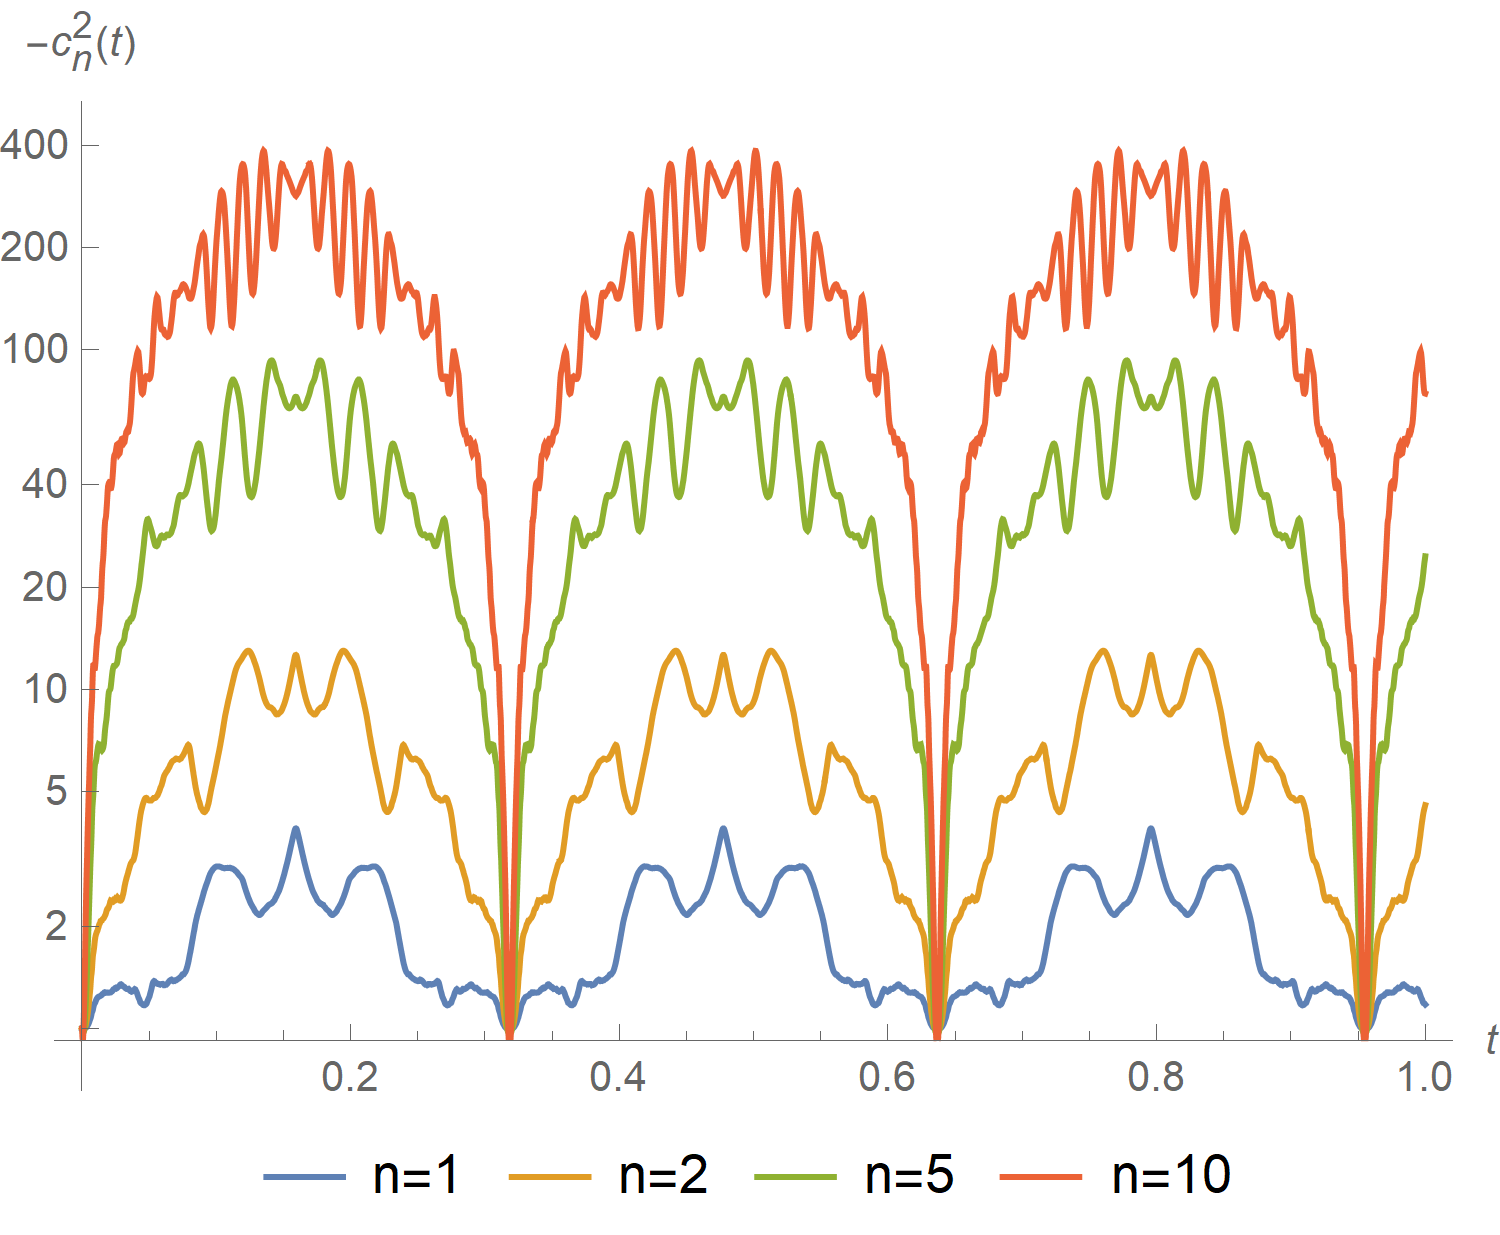
\includegraphics[width=0.8\textwidth]{microcanonicalwell}
\caption{Microcanonical out-of-time-order correlators for the particle in a 1D box (L=1) (See \cite{Hashimoto_2017}, figure 2)}
\end{figure}
\begin{figure}
\centering
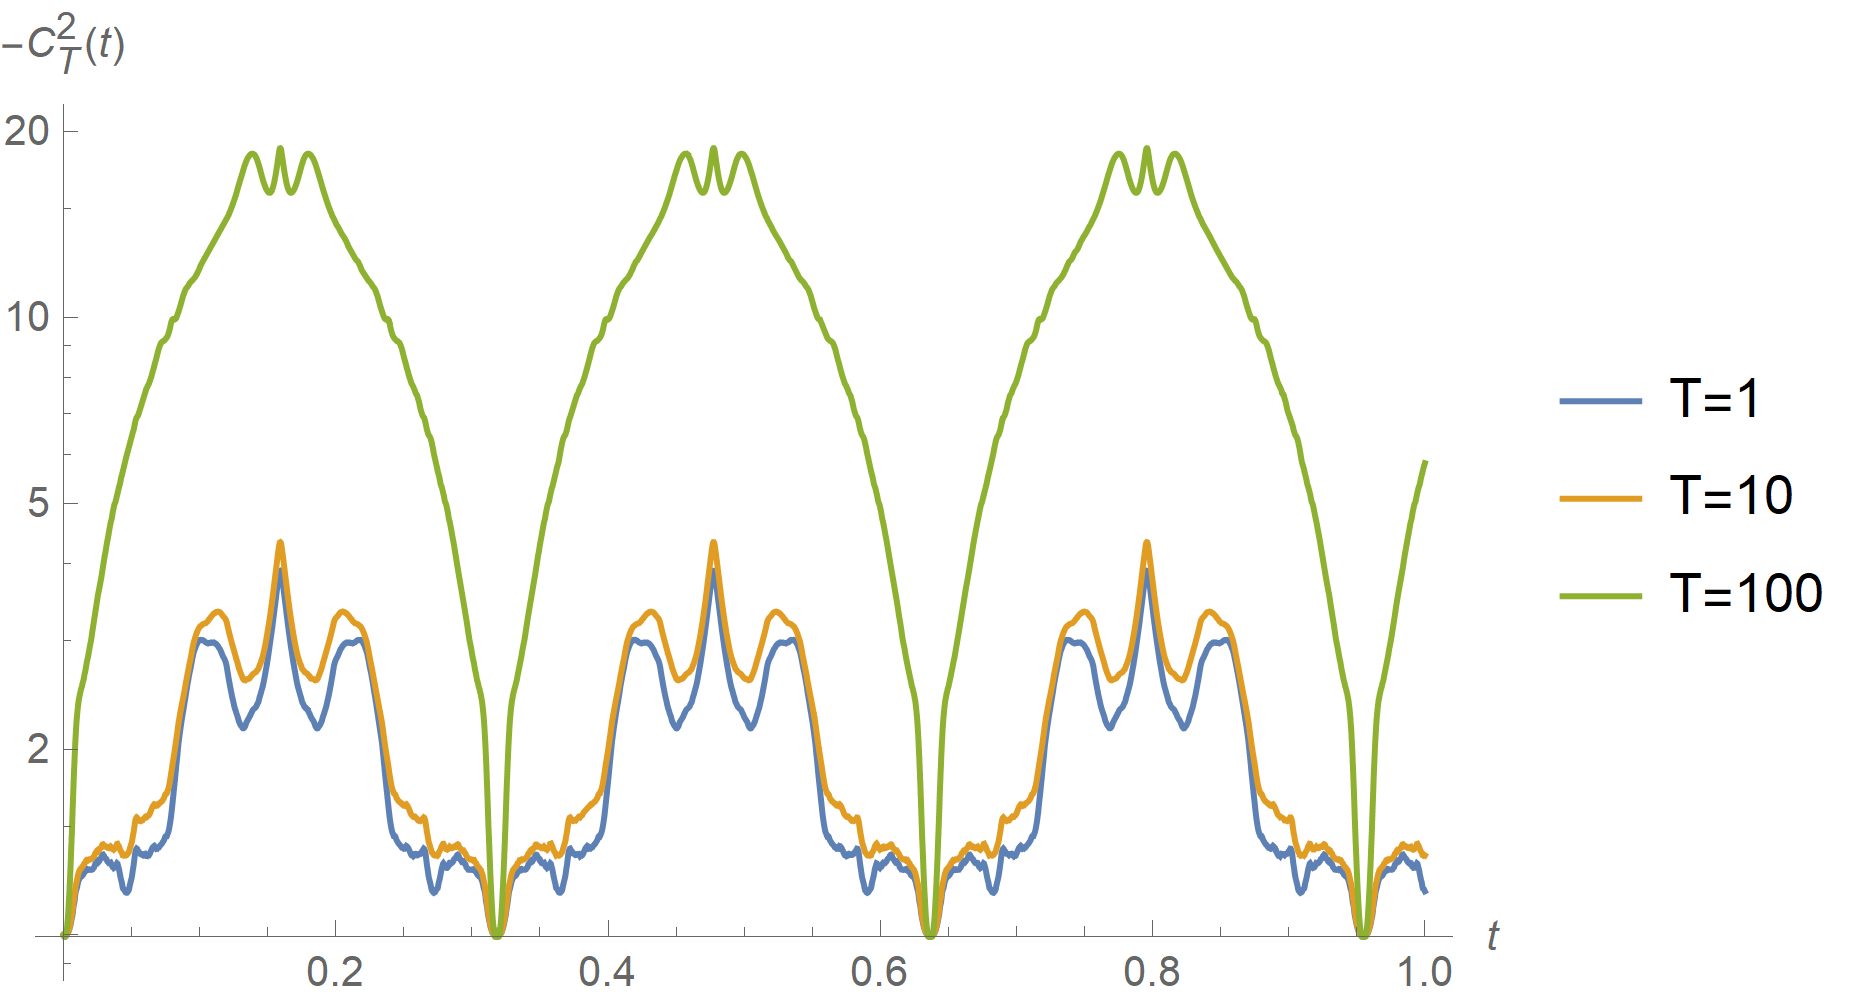
\includegraphics[width=0.8\textwidth]{macrocanonicalwell}
\caption{Macrocanonical OTOCs for the particle in a 1D box (L=1)}
\end{figure}
\begin{figure}
\centering
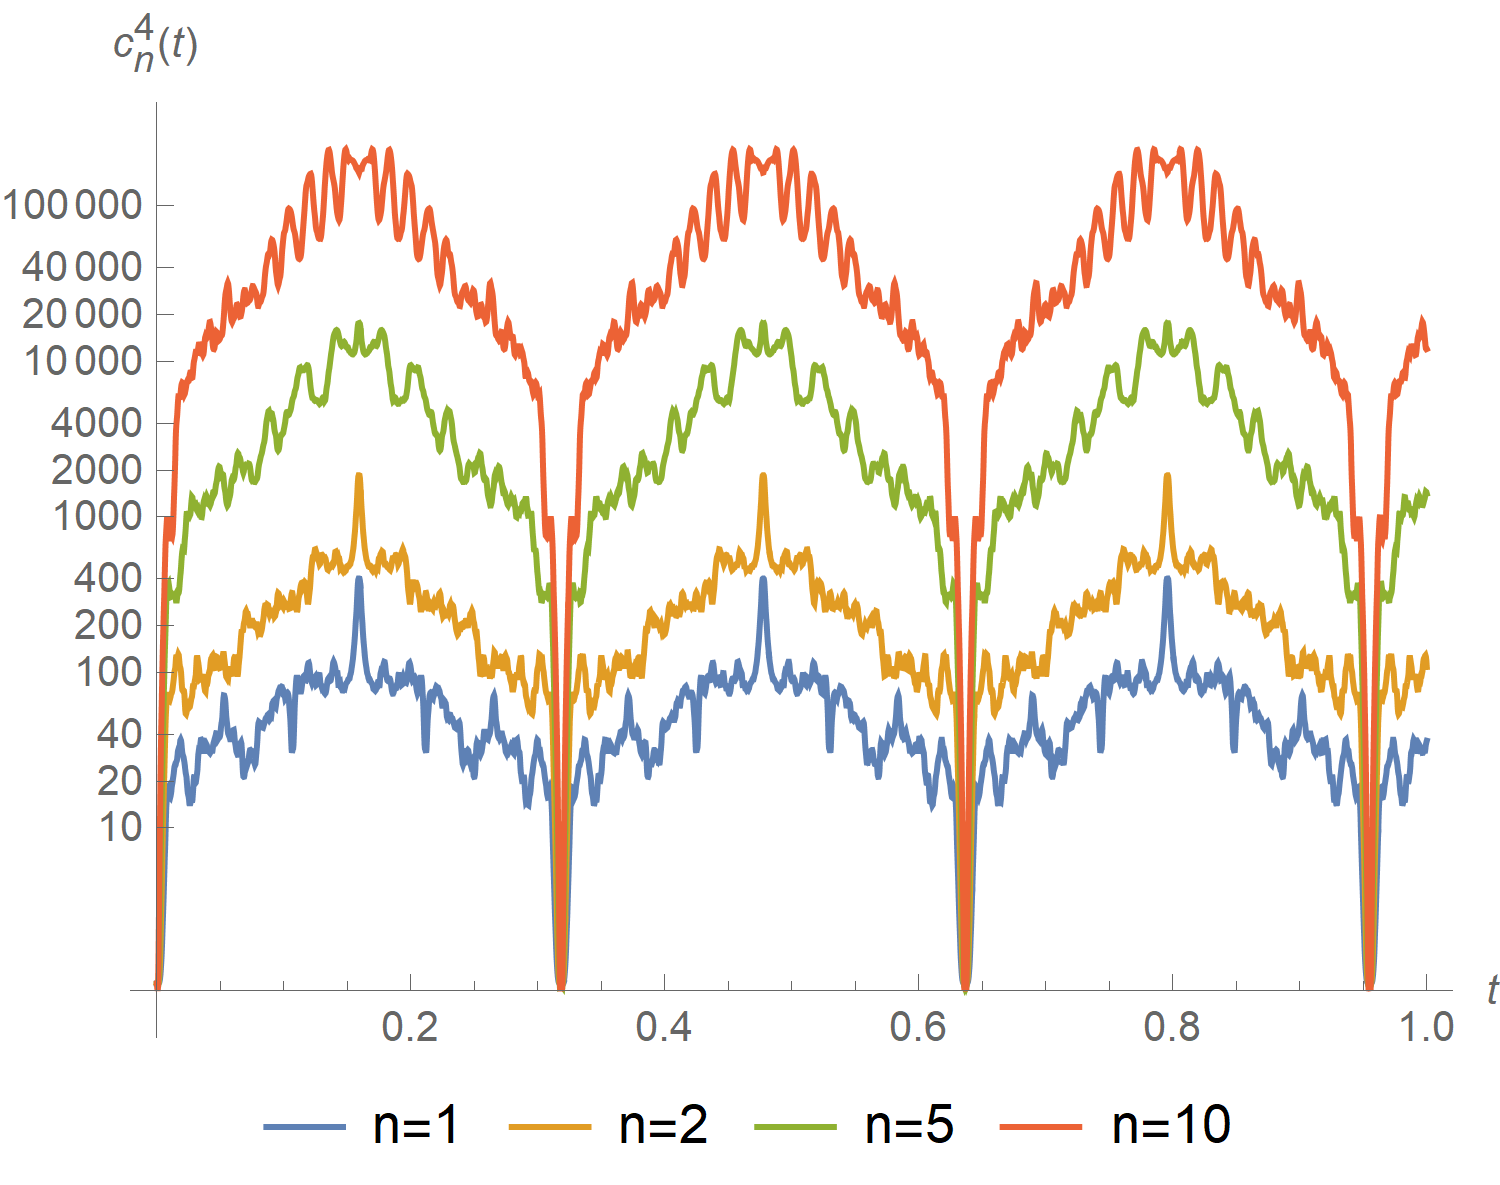
\includegraphics[width=0.4\textwidth]{macrocanonicalwell4}
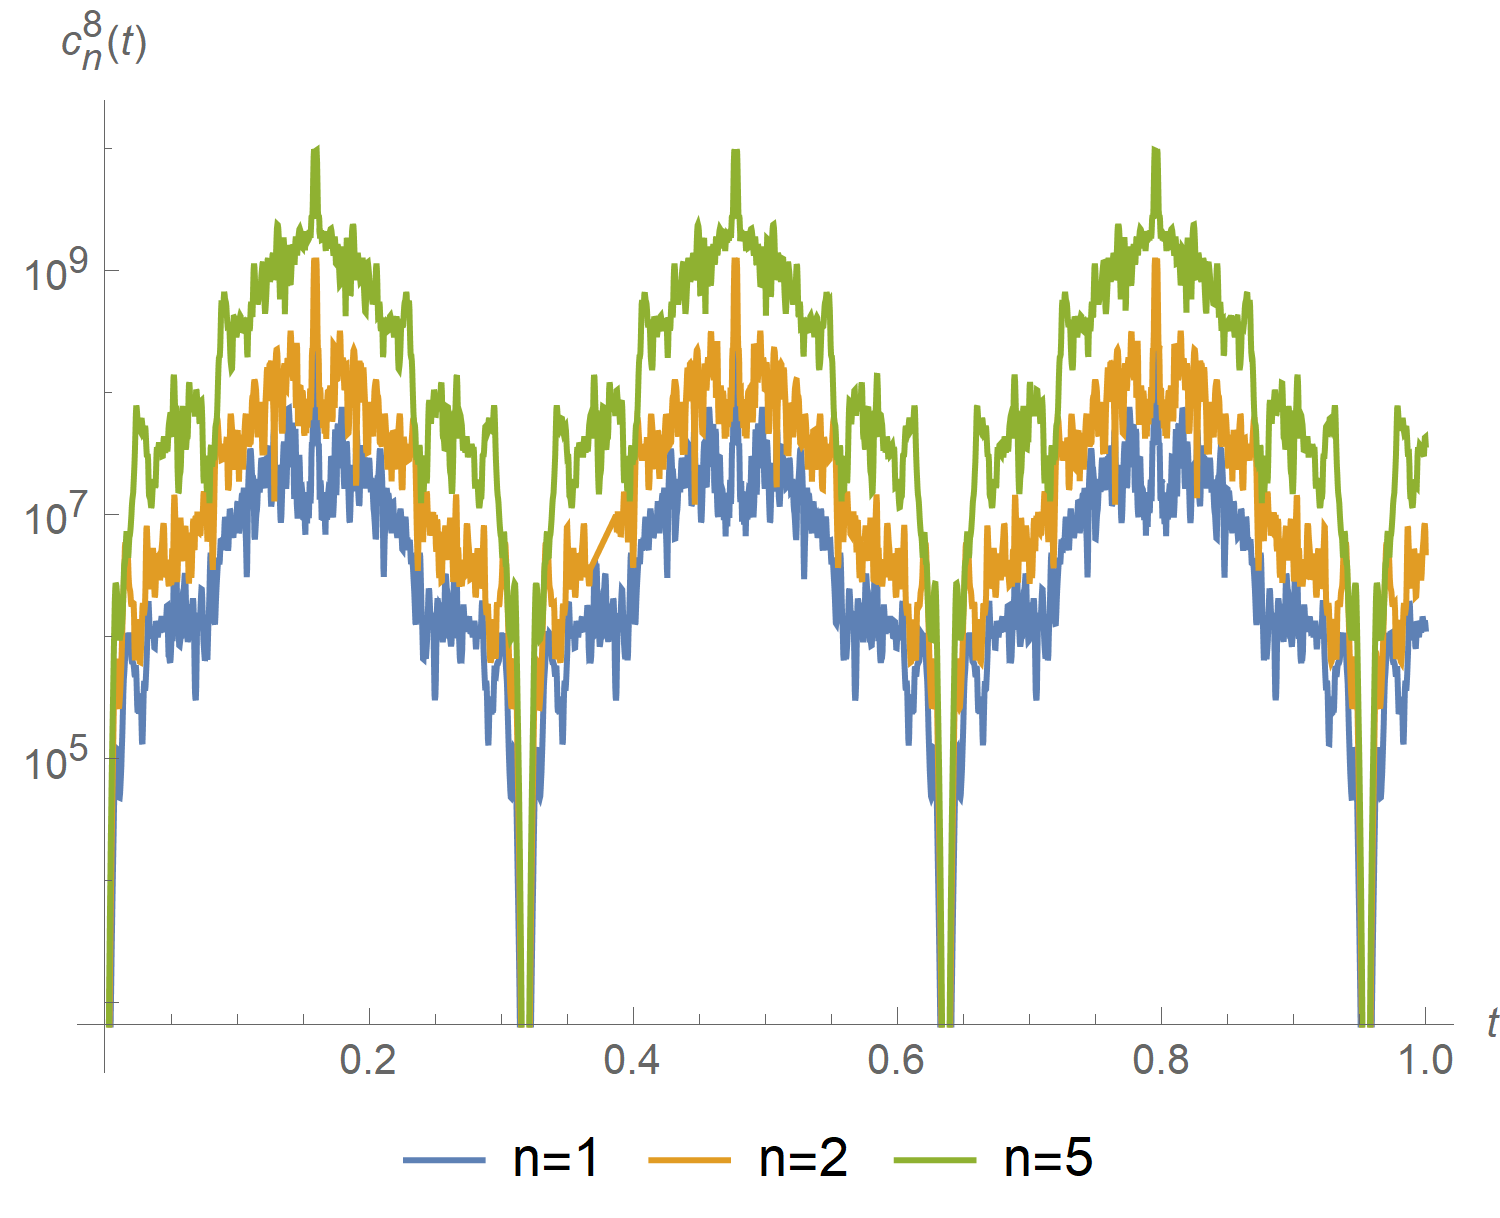
\includegraphics[width=0.4\textwidth]{macrocanonicalwell8}
\caption{Macrocanonical OTOCs $C_T^N(t)$ for $N = 4$ and 8}
\end{figure}
\begin{figure}
\centering
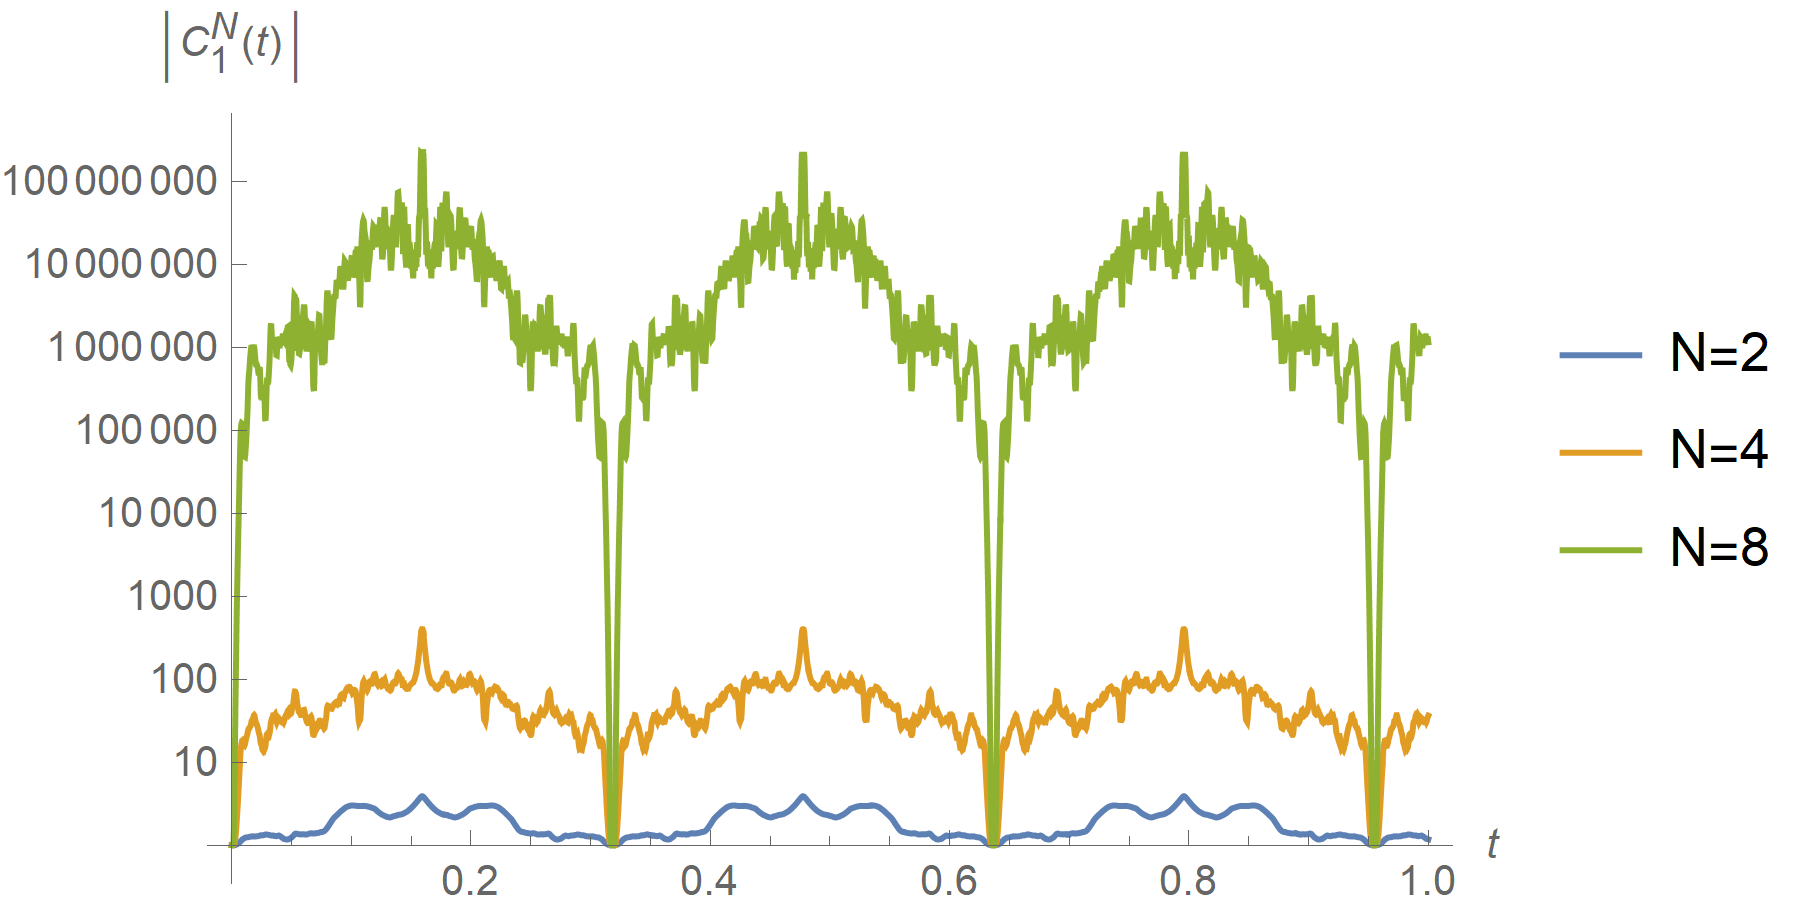
\includegraphics[width=0.8\textwidth]{macrocanonicalwellN}
\caption{Macrocanonical OTOCs $C_T^N(t)$ for $T$ fixed equal to 1 and $N$ varying for particle in a box. Note that the order of magnitude grows roughly like $N$, implying the behavior of $C_1^N$ is roughly of the form $\e^{\lambda N}$ for some $\lambda$.}
\end{figure}

\subsection{The Free Particle}

We will now calculate the micro and macrocanonical OTOCs for the free particle. Note that the strategy we have been using until now does not work because the free particle does not have a discrete spectrum. As such, we will have to resort to the definition.

First, we recall the (continuous) spectrum of the free particle, indexed by momentum, which we will call $\lambda$ as not to confuse it with the momentum operator $p$. Consequently, $\ket \lambda$ is to be understood as the eigenstate satisfying $p \ket \lambda = \lambda \ket \lambda$.
\begin{gather*}
E_\lambda = \frac1{2m} p^2\\
\psi_\lambda(x) = \braket{x|\lambda} = \frac1{\sqrt{2\pi}} \e^{\frac\I\hbar p x}
\end{gather*}

In this case, the OTOCs are given by the integral
\begin{equation}
C_T^N(t) = -\frac1Z \int \e^{-\frac1{2m} \beta \lambda^2} \braket{\lambda|[x(t),p]^N|\lambda} \dl \lambda.
\end{equation}

To calculate it, we will use several resolutions of identity, yielding
\begin{gather}
C_T^N(t) = -\frac1Z \int \e^{-\frac1{2m} \beta \lambda^2} c_\lambda^N(t) \dl \lambda,\\
c_\lambda^N(t) = \idotsint \dl \lambda_1 \dots \dl \lambda_{N-1} b_{\lambda \lambda_1} \dots b_{\lambda_{N-1} \lambda},\\
b_{\lambda_1 \lambda_2} = \braket{\lambda_1 | [x(t), p] | \lambda_2}.
\end{gather}

We will now calculate $b_{\lambda_1 \lambda_2}$ explicitly. The first step is to expand
\begin{multline}
b_{\lambda_1 \lambda_2} = \braket{\lambda_1 | U(-t) x U(t) p | \lambda_2} - \braket{\lambda_1 | p U(-t) x U(t) | \lambda_2}\\
= \frac1{2m} (\lambda_2^2 - \lambda_1^2) \braket{\lambda_1 | U(-t) x U(t) | \lambda_2},
\end{multline}
so the problem is reduced to calculating $\braket{\lambda_1 | U(-t) x U(t) | \lambda_2}$. To do so, begin by calculating the wavefunction of $U(t) \ket{\lambda_2}$:
\begin{equation}
\e^{-\frac\I\hbar H} \ket{\lambda_2} = \e^{-\frac\I{2 m \hbar} \lambda_2^2} \ket{\lambda_2},
\end{equation}
and so we conclude
\begin{equation}
b_{\lambda_1 \lambda_2} \frac1{2m} (\lambda_2^2 - \lambda_1^2) \e^{-\frac\I{2 m \hbar} (\lambda_2^2 - \lambda_1^2)} \braket{\lambda_1 | x | \lambda_2}.
\end{equation}

Finally, we could try to calculate $\braket{\lambda_1 | x | \lambda_2}$ explicitly by integrating, but that would result in an oscillatory integral that doesn't seem to converge. As such, we resort to the following shortcut:
\begin{multline}
\frac1{2m} (\lambda_2^2 - \lambda_1^2) \braket{\lambda_1 | x | \lambda_2} = \braket{\lambda_1 | x p | \lambda_2} - \braket{\lambda_1 | p x | \lambda_2}\\
= \braket{\lambda_1 | [x,p] | \lambda_2} = - \I \hbar \braket{\lambda_1 | \lambda_2}.
\end{multline}

Therefore, we conclude that
\begin{equation}
b_{\lambda_1\lambda_2} = - \I \hbar \e^{-\frac\I{2m\hbar}(\lambda_2^2 - \lambda_1^2)} \braket{\lambda_1 | \lambda_2},
\end{equation}
and so
\begin{multline}
c_\lambda^N(t) = \idotsint \dl \lambda_1 \dots \dl \lambda_{N-1} b_{\lambda \lambda_1} \dots b_{\lambda_{N-1} \lambda}\\
= (-\I \hbar)^N \idotsint \dl \lambda_1 \dots \dl \lambda_{N-1} \braket{\lambda|\lambda_1} \dots \braket{\lambda_{N-1}|\lambda} = (-\I\hbar)^N \braket{\lambda|\lambda}.
\end{multline}

The quantity $\braket{\lambda|\lambda}$ is the norm of the eigenstate $\ket \lambda$, which is not a normalizable state, so technically $\braket{\lambda|\lambda}$ is infinite. However, in what follows, we will act as though it is a real constant.

Now, we can easily calculate the macrocanonical OTOC:
\begin{multline}
C_T^N(t) = -\frac1Z \int \e^{- \beta E_\lambda} c_\lambda^N(t) \dl \lambda = - \frac1Z (-\I\hbar)^N \int \e^{- \beta E_\lambda} \dl \lambda \braket{\lambda|\lambda}\\
= - \frac1Z (-\I\hbar)^N Z \braket{\lambda|\lambda} = - (-\I\hbar)^N \braket{\lambda|\lambda}.
\end{multline}

In other words, for practical purposes, the OTOCs of the free particle are all constant. Note the term $-(-\I\hbar)^N$, which is also present in the OTOCs of the Harmonic Oscillator.

\section{In which I attempt to find estimates for $C_T^N(t)$ for large $N$ (and fail)}

\subsection{Setting up an ODE}

Recall the auxilliary variables we used to calculate OTOCs:
\begin{gather}
C_T^N(t) = -\frac1Z \sum \e^{-\beta E_n} c_n^N(t),\tag{\ref{bigcdef}}\\
c_n^N(t) = \braket{n|[x(t), p]^N|n} = \sum_{k_1, \dots, k_{N-1}} b_{nk_1} b_{k_1 k_2} \dots b_{k_{N-1} n}, \tag{\ref{smallcdef}}\\
b_{ij} = \braket{i|[x(t), p]|j}. \tag{\ref{bdef}}
\end{gather}

Let us further add the auxilliary variable
\begin{equation}
\sigma_{ij}^N(t) = \left(\frac\I\hbar\right)^N \sum_{k_1, \dots, k_{N-1}} \braket{i|[x(t/N), p]|k_1} \dots \braket{k_{N-1}|[x(t/N), p]|j}.
\end{equation}

Then, we can use $\sigma_{ij}^N(t)$ to write $c_n^N(t)$
\begin{equation}
c_n^N(t) = \sigma_{ij}^N(t N),
\end{equation}
and we can find an easy recurrence relation for $\sigma_{ij}^N(t)$
\begin{equation}
\sigma_{ij}^{N+1}(t + \frac1{N+1} t) =  \frac\I\hbar \sum_{k} \sigma_{ik}^N(t) \braket{k|[x(\frac1{N+1} t), p]|j},
\end{equation}
which can be rearranged into
\begin{multline}
\frac{\sigma_{ij}^{N+1}(t + \frac1{N+1} t) - \sigma_{ij}^{N+1}(t)}{t/(N+1)} + \frac{\sigma_{ij}^{N+1}(t) - \sigma_{ij}^{N}(t)}{t/(N+1)}\\
= \sigma_{ij}(t) \frac{\tfrac\I\hbar \braket{j|[x(\frac1{N+1} t), p]|j} - 1}{t/(N+1)} + \frac\I\hbar \sum_{k \neq j} \tfrac{N+1}t \sigma_{ik}^N(t) \braket{k|[x(\tfrac1{N+1} t), p]|j}.
\end{multline}

Assuming that $\sigma_{ij}^N(t)$ converges fast enough to some limit $\sigma_{ij}(t)$, the second term can be neglected, yielding
\begin{multline}
\frac{\sigma_{ij}^{N+1}(t + \frac1{N+1} t) - \sigma_{ij}^{N+1}(t)}{t/(N+1)}\\
= \sigma_{ij}(t) \frac{\tfrac\I\hbar \braket{j|[x(\frac1{N+1} t), p]|j} - 1}{t/(N+1)} + \frac\I\hbar \sum_{k \neq j} \tfrac{N+1}t \sigma_{ik}^N(t) \braket{k|[x(\tfrac1{N+1} t), p]|j},
\end{multline}
and in the large $N$ limit this can be seen as a linear differential equation
\begin{equation}
\begin{cases}
\diff{\sigma_{ij}(t)}t  = \sum_{k} \frac\I\hbar \diff{\braket{k|[x(s), p]|j}}s[0] \sigma_{ik}(t),\\
\sigma_{ij}(0) = \delta_{ij}.
\end{cases}
\end{equation}

Unfortunately, this does not work particularly well, and in retrospect there is no reason to expect it should. For example, the limit $\sigma_{ij}^N(t)$, $N \to \infty$, does not necessarily exist. If we look at the figures for the infinite well, the OTOCs grow exponentially with N. Furthermore, also in the infinite well, the derivatives $\diff{\braket{k|[x(s), p]|j}}s[0]$ don't seem to exist. In fact, I've verified an odd phenomenon wherein the limit
\begin{equation}
\lim_{s \to 0} \frac{\braket{k|[x(s), p]|j} - \braket{k|[x, p]|j}}{s}
\end{equation}
is zero, but if the denominator is replaced by $s^{3/2}$ then the lateral limits
\begin{equation}
\lim_{s \to 0^\pm} \frac{\braket{k|[x(s), p]|j} - \braket{k|[x, p]|j}}{s^{3/2}}
\end{equation}
exist and are non-null, implying that $\braket{k|[x(s), p]|j}$ behaves near $s=0$ like $\braket{k|[x, p]|j} + K_\pm s^{3/2}$, which has null first derivative and infinite second derivative. It could be worth investigating this phenomenon, but I've decided that's beyond the scope of what I'm trying to do. In any case, this implies in particular that any attempt at a first-order approximation of OTOCs near the origin is not likely to work, at least for cases such as the infinite well.

\begin{figure}
\centering
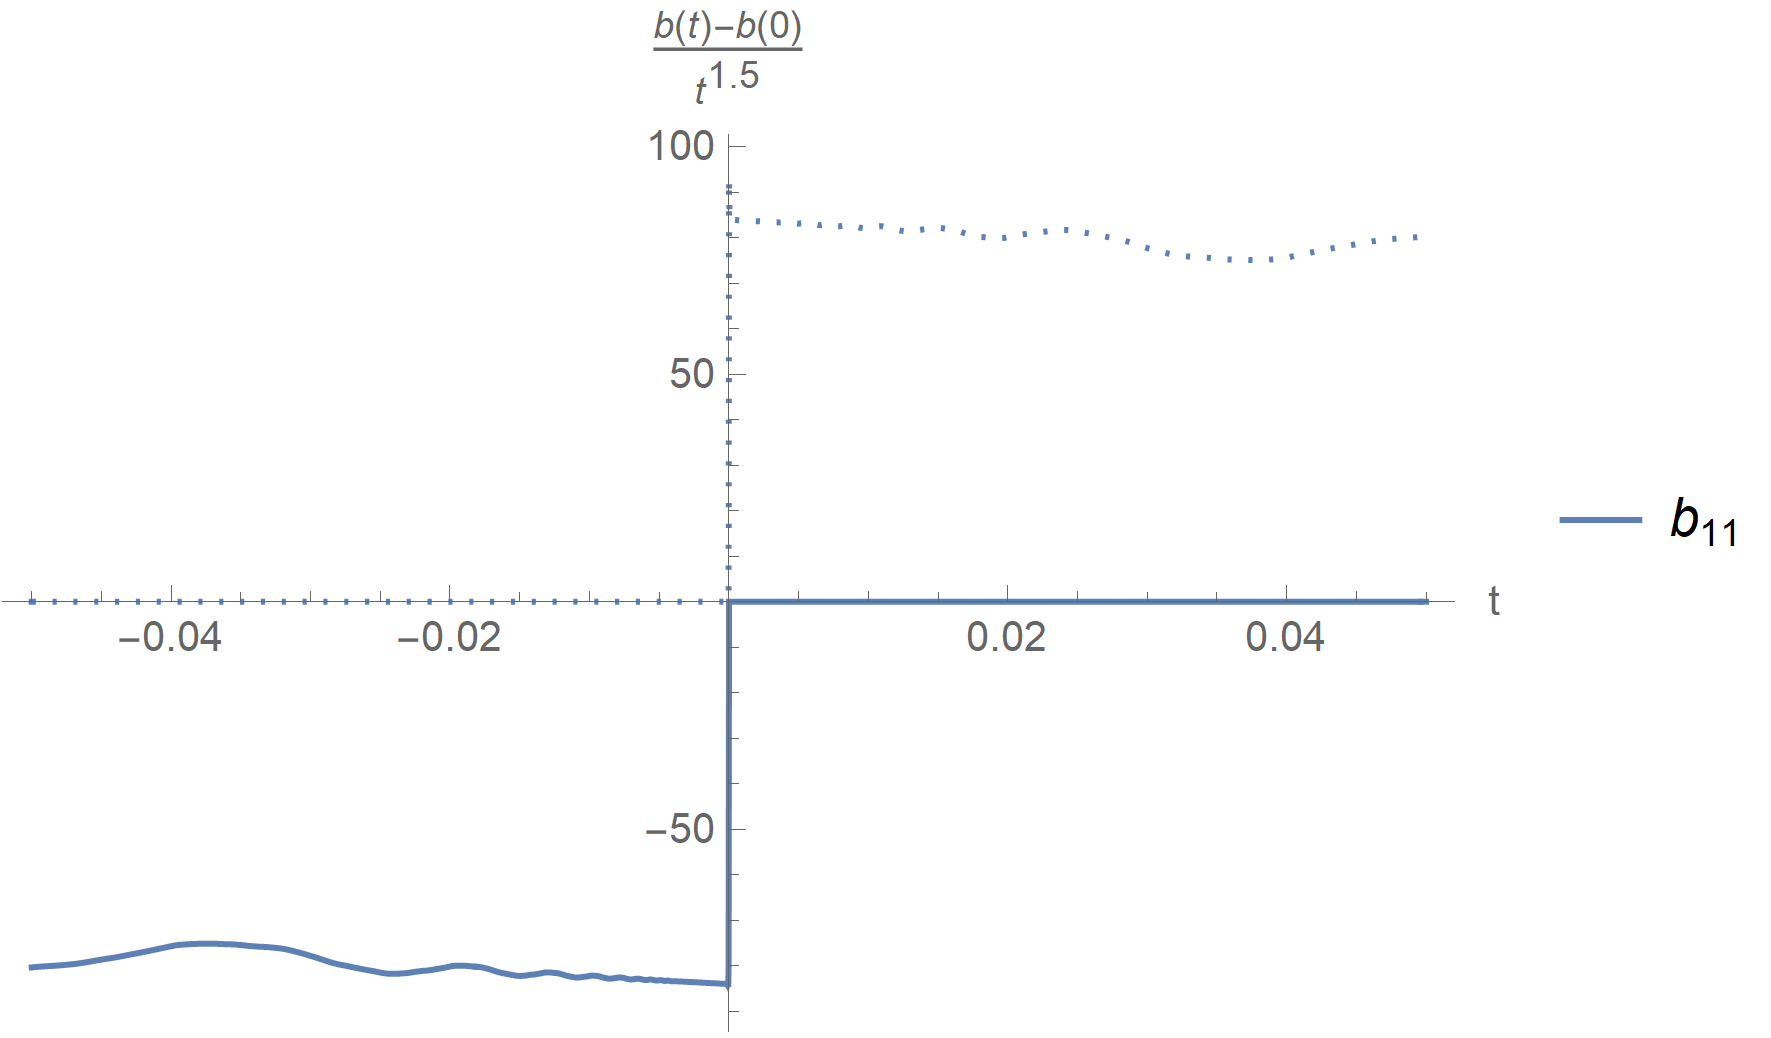
\includegraphics[width=0.8\textwidth]{pseudoderivativeb11}
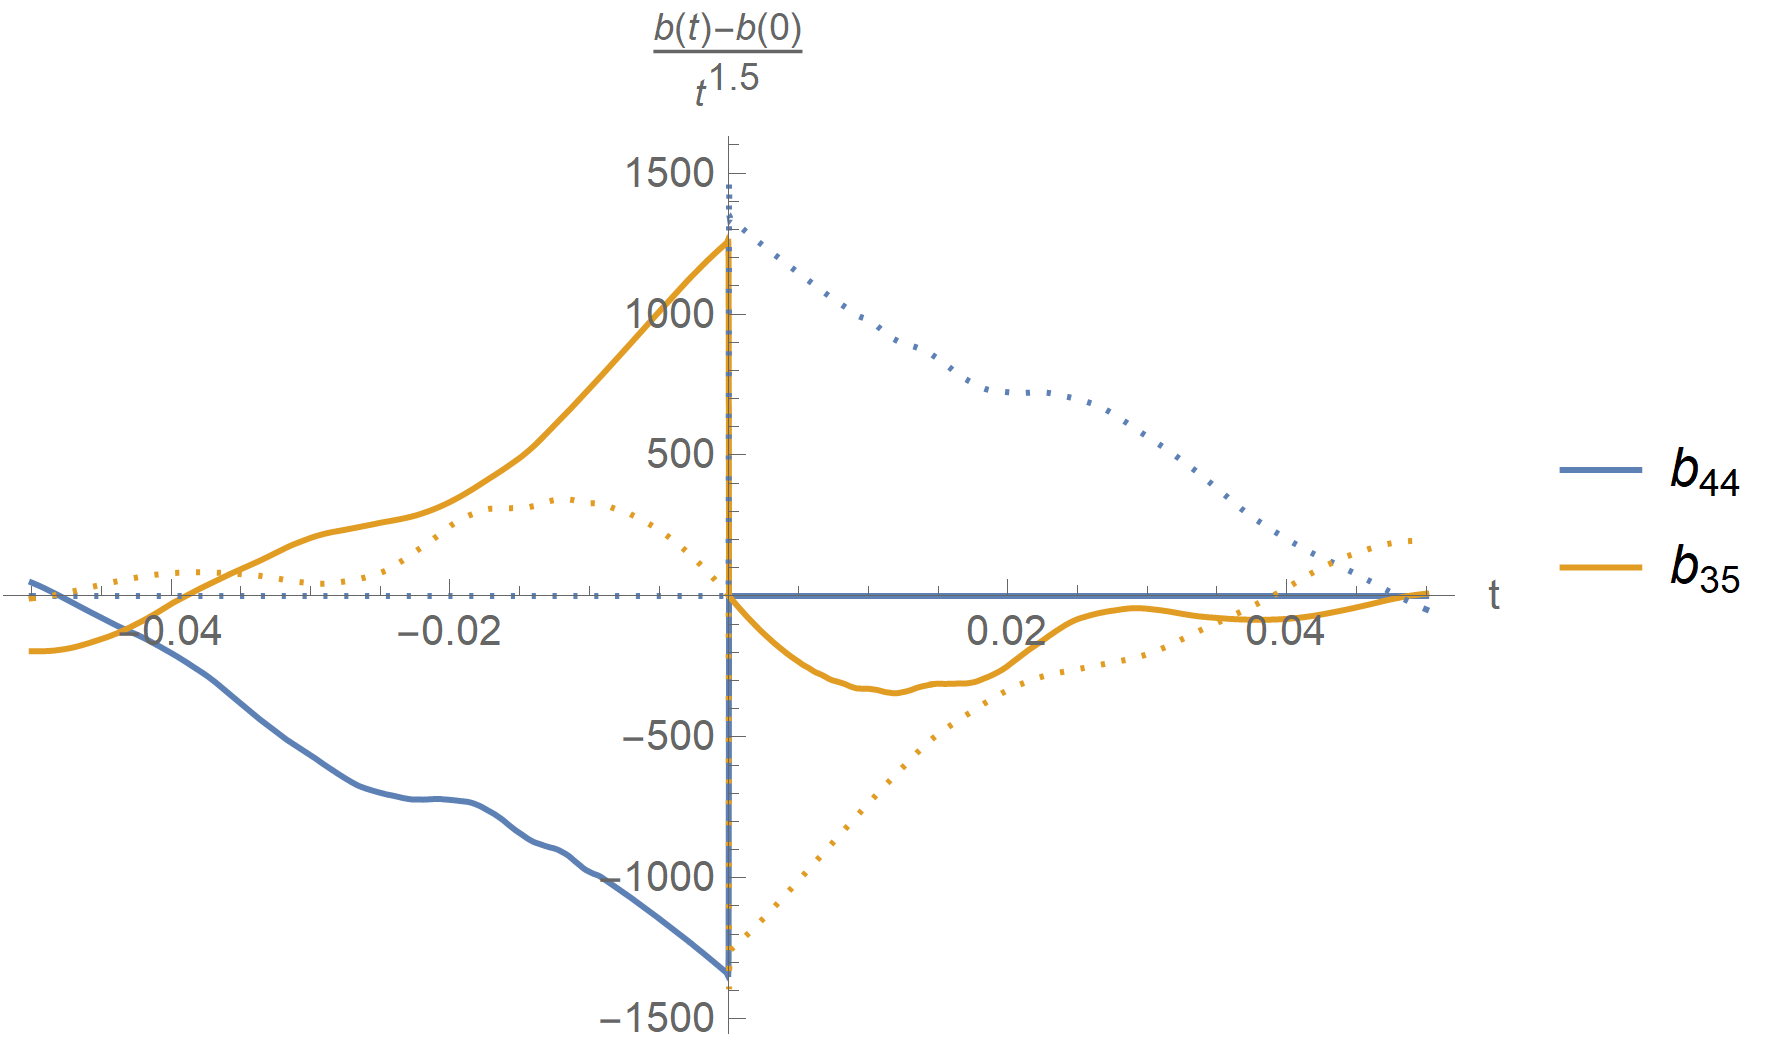
\includegraphics[width=0.8\textwidth]{pseudoderivativeb4435}
\caption{Existence of `pseudo-derivatives' of $b_{ij}(t)$ for a few pairs $i$, $j$. Full lines represent real part, dashed lines represent imaginary part. It is clear from the graphs that $\lim_{s \to 0^\pm} \frac{\braket{k|[x(s), p]|j} - \braket{k|[x, p]|j}}{s^{3/2}}$ exists.}
\end{figure}

\subsection{Calculating through path integrals}

In the previous subsection, we saw that trying to approximate OTOCs using
\begin{equation}
\sigma_{ij}^N(t) = \left(\frac\I\hbar\right)^N \sum_{k_1, \dots, k_{N-1}} \braket{i|[x(\tfrac t N), p]|k_1} \dots \braket{k_{N-1}|[x(\tfrac t N), p]|j}
\end{equation}
is not likely to work if we try to approximate each term $\braket{i|[x(\tfrac t N), p]|j}$ in first order, because the first order approximation might not exist near zero. However, if we replaced Hamiltonian eigenstates by position eigenstates, we would get an expression of the form
\begin{multline}
\sigma_{q q'}^N(t) = \left(\frac\I\hbar\right)^N \braket{q|[x(\tfrac t N), p]^N|q'}\\
= \left(\frac\I\hbar\right)^N \idotsint \dl q_1 \dots \dl q_N \braket{q|[x(\tfrac t N), p]|q_1} \dots \braket{q_{N}|[x(\tfrac t N), p]|q'}
\end{multline}
from which the OTOC can be recovered, as
\begin{multline}
c_n^N(t) = \iint \dl q \dl q' \braket{n|q} \braket{q|[x(t), p]^N|q'} \braket{q'|n}\\
= (-\I \hbar)^N \iint \dl q \dl q' \psi_n^*(q) \psi_n(q') \sigma_{qq'}^N(N t).
\end{multline}

Therefore, it is worth investigating if $\sigma^N_{qq'}(t)$ converges as $N \to \infty$, and if so it would be plausible to think that it could be written as a path integral of the form
\begin{equation}
\sigma_{q q'}^\infty(t) = \int_{q(0) = q}^{q(t) = q'} [\dl q(s)] F(q),
\end{equation}
for some functional $F$.

Unfortunately, this approach failed in the crib, when I tried to calculate a single term of the form $\braket{q|[x(t),p]|q'}$ for the Harmonic Oscillator. I will now show my calculations.

To begin, we can separate the commutator
\begin{equation}
\braket{q|[x(t),p]|q'} = \braket{q | U(-t) x U(t) p | q'} - \braket{q | p U(-t) x U(t) | q'}.
\end{equation}

Now, let us calculate $U(-t)xU(t)\ket{q'}$, one part at a time. The first part, $U(t) \ket{q'}$ is easy, as the Harmonic Oscillator has a Gaussian Lagrangian, and we calculated the propagator for Gaussian Lagrangians in class. Indeed,
\begin{equation}
\braket{y|U(t)|q'} = K(q',y|t) = \sqrt{\frac{m \omega}{2 \I \pi \hbar \sin(\omega t)}} \e^{\frac\I\hbar S_c},
\end{equation}
where $S_c$ is the classical action. This can be readily calculated for the Harmonic Oscillator as
\begin{equation}
S_c(q', y; t) = \frac1{2 \sin(\omega t)} \omega m (y^2 \cos(\omega t) - 2 q' y + q'^2 \cos(\omega t)),
\end{equation}
and therefore we conclude
\begin{gather}
\braket{y|U(t)|q'} = \sqrt{\frac{m \omega}{2 \I \pi \hbar \sin(\omega t)}} \e^{\frac\I\hbar \frac1{2 \sin(\omega t)} \omega m (y^2 \cos(\omega t) - 2 q' y + q'^2 \cos(\omega t))},\\
\braket{y| x U(t)|q'} = y \sqrt{\frac{m \omega}{2 \I \pi \hbar \sin(\omega t)}} \e^{\frac\I\hbar \frac1{2 \sin(\omega t)} \omega m (y^2 \cos(\omega t) - 2 q' y + q'^2 \cos(\omega t))}.
\end{gather}

Finally, it is necessary to compute $U(-t) x U(t) \ket{q'}$. The way to go would appear to be through a resolution of identity
\begin{equation}
\begin{aligned}
\braket{y|U(-t) x U(t) | q'} &= \int \dl z \braket{y|U(-t)|z} \braket{z|x U(t)|q'}\\
&\begin{multlined}
= \int \dl z  \sqrt{\frac{\I m \omega}{2 \pi \hbar \sin(\omega t)}} \e^{-\frac\I\hbar \frac1{2 \sin(\omega t)} \omega m (z^2 \cos(\omega t) - 2 z y + y^2 \cos(\omega t))} \times\\
\times z \sqrt{\frac{m \omega}{2 \I \pi \hbar \sin(\omega t)}} \e^{\frac\I\hbar \frac1{2 \sin(\omega t)} \omega m (z^2 \cos(\omega t) - 2 q' z + q'^2 \cos(\omega t))}
\end{multlined}\\
&\begin{multlined}
= \int \dl z  z \frac{m \omega}{2 \pi \hbar \sin(\omega t)} \e^{\frac\I\hbar \frac1{2 \sin(\omega t)} \omega m (-z^2 \cos(\omega t) + 2 z y - y^2 \cos(\omega t))} \times\\
\times \e^{\frac\I\hbar \frac1{2 \sin(\omega t)} \omega m (z^2 \cos(\omega t) - 2 q' z + q'^2 \cos(\omega t))}
\end{multlined}\\
&= \e^{\frac\I\hbar \frac1{2} \tg(\omega t) \omega m (q'^2 - y^2)} \int \dl z  z \frac{m \omega}{2 \pi \hbar \sin(\omega t)} \e^{-\frac\I\hbar \frac1{ \sin(\omega t)} \omega m (y-q') z},
\end{aligned}\label{badintegrand}
\end{equation}
and now we reach an impasse, because the integrand is not integrable. It is an oscillatory integral, but one whose oscillations always have the same frequency, and whose amplitude only increases as one goes towards infinity. See figure \ref{badplot}.

\begin{figure}
\centering
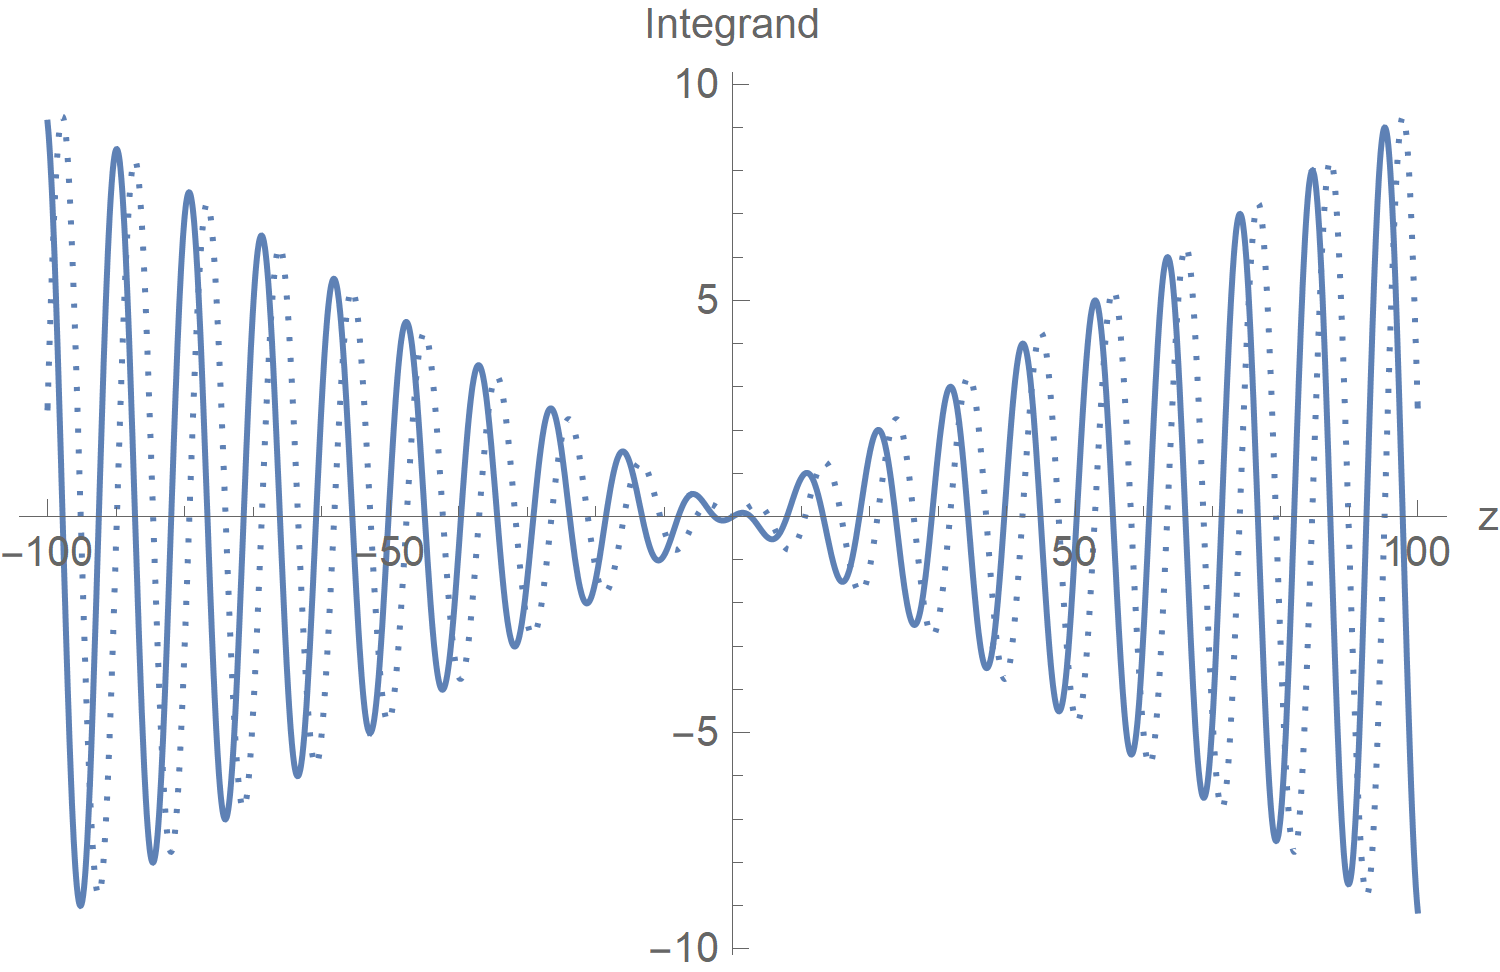
\includegraphics[width=0.8\textwidth]{badplot}
\caption{Plot of the integrand of \eqref{badintegrand} with $z$ left variable and all other parameters fixed arbitrarily}
\label{badplot}
\end{figure}

Regardless of this unfortunate state of affairs, there is something that can be done to try to calculate \eqref{badintegrand}. Even though mathematically it doesn't make sense to apply integration by parts in this case, if it works it works, right?
\begin{multline}
\int \dl z  z \frac{m \omega}{2 \pi \hbar \sin(\omega t)} \e^{-\frac\I\hbar \frac1{ \sin(\omega t)} \omega m (y-q') z}\\
= \int \dl z \frac{\I}{(y-q')} \frac{1}{2 \pi} \e^{-\frac\I\hbar \frac1{ \sin(\omega t)} \omega m (y-q') z}.
\end{multline}

This is still an unpleasant situation, but at least there is a way forward. Indeed, if $y \neq q'$ this is an imaginary exponential, which `has null average value'. On the other hand, if $y = q'$, this is the integral of a constant, which `is infinity'. Therefore, this can be seen as a Dirac delta, and by analogy with computations like $\braket{x|x}$ and $\braket{p|p}$ it seems reasonable to assume that the factor of $2\pi$ vanishes when we consider this as a Dirac delta. Therefore, I predict that
\begin{equation}
\braket{y|U(-t) x U(t) | q'} = \e^{\frac\I\hbar \frac1{2} \tg(\omega t) \omega m (q'^2 - y^2)} \frac\I{y-q'} \braket{y|q'}.
\end{equation}

Unfortunately, not only have these computations been founded on very shaky mathematics, but they also don't seem to get me any closer to calculating $\braket{q|[x(t),p]|q'}$, because I would need to apply $p$ to this result and I don't know enough about distribution theory to proceed. Therefore, I have given up on approximating the OTOCs through path integration.

\nocite{Hashimoto_2017}
\nocite{romatschke2021quantum}

\bibliographystyle{plain}
\bibliography{bibliography}

\end{document}